\documentclass{article}
\usepackage{graphicx} % Required for inserting images
\usepackage{xcolor}
\usepackage{enumitem}
\usepackage{amsmath}
\usepackage{tikz}
\usepackage{fullpage}
\usepackage{mathtools}

\usetikzlibrary{arrows,shadows,positioning}
\usepackage{pgf-umlsd}

\newcounter{diagram}
\newcounter{step}
\counterwithin*{step}{diagram}
\newcommand\nextstep{\refstepcounter{step}\thestep: }
\newcommand\resetstep{\refstepcounter{diagram}}

\newcommand{\ramc}[1]{\textcolor{cyan}{#1}}
\newcommand{\eepromc}[1]{\textcolor{red}{#1}}
\newcommand{\ramt}[1]{#1}
\newcommand{\eepromt}[1]{#1}

% \bibliographystyle{plain}
% \usepackage[style=numeric,backend=biber,sorting=none]{biblatex}
% \addbibresource{refs.bib}

\usepackage[breaklinks,hyperindex,colorlinks,anchorcolor=black,citecolor=black,filecolor=black,linkcolor=black,menucolor=black,urlcolor=black,pdftex]{hyperref}


\definecolor{midblue}{rgb}{0,0,.7}
\hypersetup{
  colorlinks=true,
  linkcolor=midblue,
  citecolor=midblue,
  urlcolor=midblue
}

\title{Security Protocol Project \\ \Large{Design Proposal}}
\author{Felix M\"older \\ s1022118
\and Maximilian Pohl \\ s1103073
\and Bart Veldman \\ s1017975}
\date{\today}

\begin{document}

\maketitle

% Project Information sheet:
% http://www.cs.ru.nl/~erikpoll/spp/javacard_project.pdf


\section{Use Cases}
Our group decided to design, develop and implement an electronic purse system.
This system consists of the following components:
\begin{itemize}
    \item Smart cards
    \item Reload terminals
    \item POS (point-of-sale) terminals
    \item Initialization terminals
    \item A back end
\end{itemize}
The issuer of the cards uses the initialization terminal to initialize a new card and deliver the initialized card to the end user.
At every reload terminal, the user can load money on their smart card and can pay for goods and services at every POS terminal that salesmen supply.
An example application for this system is a university canteen.
Students can load money on their student cards at reload terminals.
Later, they can pay for lunch and food at the POS terminals in the university canteen.
We will define the following use cases:
\begin{enumerate}[label={UC\arabic*:}, ref={UC\arabic*}, leftmargin=3\parindent]
    \item \label{uc:person} The card is initialized at an initialization terminal once before being provided to the end user.
    
    \item \label{uc:reload} At a reload terminal, the end user can increase the balance of the smart card by paying with cash or with a bank card.
    
    \item \label{uc:payment} At the POS terminal, the end user can pay for goods and services with the smart card.
    A user can use a POS terminal, even if the terminal is not connected to the back end (offline).

    \item A POS or reload terminal can be deactivated remotely with some delay (e.g., one week).
    
    \item The end user can declare the card as lost or stolen, which results in the card being blocked.
    For the sake of simplicity of the protocol, we do not allow the unblocking of a blocked card.
    
\end{enumerate}
\subsection{Lifecycle}
The smart-card lifecycle is depicted in Figure~\ref{fig:lifecycle}.
%In the \emph{Initial} state, the smart card consists only the raw program and no user data is loaded on the card yet.
In the \emph{Initial} state, the program is already loaded on the card, but no data exist yet.
In an actual application, the possibility to upload other applets or remove existing ones would already be disabled at this stage.

By uploading the required data onto the card, the card will move to the state \emph{Personalized}.
This is done with the initialization terminal and the initialization protocol as described in Section~\ref{sec:perProtocol}.
At this stage, the card is still in possession of the card issuer.
By handing the card over to the end user, the card transits to the \emph{Issued} state.
Internally to the card, this does not make a difference to the previous state.

We decide between two end states.
Either a card gets \emph{Blocked} because it was lost or stolen, or it moves to the \emph{End-of-Live} state because it reached its expiration date or the transaction counter, which is explained later, overflows.
The two end states do not make a difference internally to the card, both result in the card refusing any interaction.
A card that is blocked or End-of-Live cannot be unblocked.

\begin{figure}
    \centering
    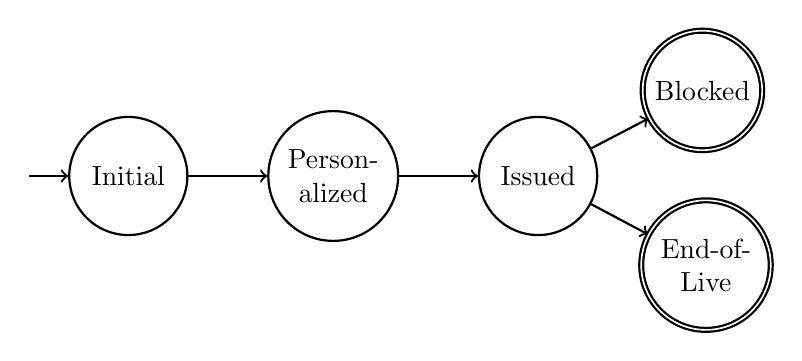
\begin{tikzpicture}[node distance=0mm and 1cm, thick, end/.style = {main, double}, main/.style = {draw, circle, align=center, minimum size=1.5cm}] 
\coordinate (start);
\node[main] (init) [right=0.5cm of start]{Initial}; 
\node[main] (person) [right=of init]{Person-\\alized}; 
\node[main] (issued) [right=of person] {Issued}; 
\node[end] (blocked) [above right=of issued] {Blocked}; 
\node[end] (eol) [below right=of issued] {End-of-\\Live};
\draw[->] (start) -- (init);
\draw[->] (init) -- (person); 
\draw[->] (person) -- (issued);
\draw[->] (issued) -- (blocked);
\draw[->] (issued) -- (eol);
\end{tikzpicture} 
    \caption{Lifecycle of the smart-card}
    \label{fig:lifecycle}
\end{figure}


\section{Attacker Model}\label{attackerModel}
To understand possible attack scenarios, we first have to list what a potential attack would like to achieve.
The goals of an attacker, i.e., the threats considered in our protocol, are:
\begin{enumerate}[label={T\arabic*:}, leftmargin=2\parindent, ref={T\arabic*}]
    \item \label{threat:increaseWithoutPaying}
    The end user is interested in increasing their balance (which is stored on the card) without actually paying for it.
    
    \item \label{threat:payWithoutDecrease}
    The end user is interested in forging a payment such that the POS terminal shows a successful transaction without the balance of the card actually decreasing.
    
    \item \label{threat:denyPayment}
    The end user is interested in denying having done a payment that actually happened, in order to get the money back.
    
    \item \label{threat:forgingPayments} The salesman is interested in forging payments by either 
    \begin{enumerate}[ref={\theenumi~\alph*}]
        \item \label{threat:inventNewPayments}
        inventing payments that never happened or
        \item \label{threat:alterPaymentDetails}
        by altering the details of payments that happened, such as the money source and destination or the amount transferred.
    \end{enumerate}
        
    \item \label{threat:chargeMoreThanDisplayed}
    The salesman is interested in charging more money than shown on the terminal display (if there is any).

    \item \label{threat:invaldTermial} A third person is interested in operating unauthorized POS terminals to collect payment proofs and get the money from the institution operating the system, e.g., by inserting the collected payment proofs into the log of a valid terminal.

    \item \label{threat:stolenCard} A third person is interested in using a stolen or lost card to pay with it at POS terminals.
\end{enumerate}

% Power:
%   Active MITM
%   card tear (pulling it out of the terminal while operating)
We assume an attacker that is able to shut down the card and the terminal at any (precise) point in time, e.g., by tearing the card out of the terminal or by removing the power supply of the terminal, respectively.
Additionally, an attacker is capable of performing an active man-in-the-middle attack.
This means it can read and alter any communication between the smart card and the terminal.

% TCB
%   Assume tamper-resistance
%   which persons do we have to trust?
On the other hand, we assume the smart cards and terminals to be tamper resistant.
This means it is not possible for an attacker to extract key material from the card or terminal, and the software and data stored are integer and cannot be changed.
Still, we do not want the security of the whole system to be compromised in case of a single failure in this assumption.

Furthermore, we have to trust the correctness of data fed to the terminals, e.g., the reload terminal being able to correctly count the cash inserted and that nobody tampers with the connection between the money counting machine and the terminal.
Likewise, we have to trust the clock signal the terminal provides to the card, as the card cannot keep track of time itself.
Moreover, we assume that communication between the back end and the terminals is secure.

We also do not specifically secure the initialization step.
Securing the initialization is not needed, as this functionality is already disabled when the card is given to the end user.
It is also impossible to create a valid card in case someone gets their hands on some uninitialized card, as this would require the knowledge of private secrets only known by the back end.
We do not even have to trust the person initializing the cards too much, as the private key of the card is generated within the card and, given that the software was not tampered with, cannot be exported.
The person thus could create a lot of cards with no money on them, which is not too interesting as a business model.


\section{Security Requirements}
Our system will adhere to the following security requirements (SRs). After each SR, we indicate which threat from Section~\ref{attackerModel} it aims to prevent.
\begin{enumerate}[label={SR\arabic*:}, ref={SR\arabic*}, leftmargin=3\parindent]
    \item \label{sr:mutualAuth}
    The card and the reload/POS terminal are mutually authenticated. (\ref{threat:increaseWithoutPaying}, \ref{threat:payWithoutDecrease}, \ref{threat:invaldTermial})
    
    \item \label{sr:messageAuth}
    The increase and decrease balance messages from the reload and POS terminal, respectively, are authenticated. (\ref{threat:increaseWithoutPaying}, \ref{threat:payWithoutDecrease}, \ref{threat:chargeMoreThanDisplayed})
    
    \item \label{sr:replayProtection}
    A message altering a card's balance is usable only once. (\ref{threat:increaseWithoutPaying}, \ref{threat:inventNewPayments})
    
    \item \label{sr:messageIntegrity}
    A breach of integrity in the communication between a card and a reload/POS terminal is noticed. (\ref{threat:increaseWithoutPaying}, \ref{threat:payWithoutDecrease}, \ref{threat:alterPaymentDetails})
    
    \item \label{sr:atomic}
    Money transfer between a card and terminal must behave atomically. (\ref{threat:increaseWithoutPaying}, \ref{threat:payWithoutDecrease})

    \item \label{sr:nonRepudiation}
    A terminal can prove a transaction being made. (\ref{threat:denyPayment})

    \item \label{sr:block}
    POS and reload terminals as well as cards can be deactivated remotely by trustful parties, i.e., the back end. (\ref{threat:invaldTermial}, \ref{threat:stolenCard})

    \item \label{sr:keyLeakage}
    When a key leaks from either a card or a terminal, the system as a whole should not be compromised. (\ref{threat:increaseWithoutPaying}--\ref{threat:invaldTermial})
\end{enumerate}

We decided against the following security requirements:
\begin{itemize}
    \item We do not encrypt the traffic between the card and the various terminals.
    The reason is that we do not see any relevant threat that would get mitigated by that, and would therefore only complicate the protocol without a real improvement.
    We are unsure if there is any legal requirement to encrypt the traffic, e.g., for privacy reasons.
    If so, the protocol needs to be modified accordingly.
    The same applies if we would use a pin to authenticate the cardholder.
    
    \item We decided against the authentication of the cardholder (e.g., by PIN protection), as we took systems like the Dutch \emph{Chipknip} or the usage of the student identity card for paying in the university canteen in Germany as a model.

    \item We do not authenticate the card to the reload terminal, as we did not figure out any threat that could be mitigated by that.
    If someone loads money on a faked, expired, or otherwise invalid card, the money would be lost, as the card cannot be used at any POS terminal.
\end{itemize}


\section{Key Distribution and Protocols}
\subsection{Notation} \label{sec:notation}
The following notation will be used throughout the section:
\begin{itemize}
    \item Private keys are lowercase
    
    \item Public keys are capitalized
    
    \item The subscript indicates the owner (c: Card, p: POS, r: Reload, b: Back end).
    At some places, the letter t is used to indicate any terminal.

    \item Unique identifiers of the cards and terminals are written as: ID$_{c/r/t}$

    \item The expiration dates are written as: expDate$_{c/r/t}$

    \item Encryption will be notated as: Enc$_{\textrm{Key}}$(Message)

    \item Decryption will be notated as: Dec$_{\textrm{Key}}$(Ciphertext)
    
    \item Computation of a hash will be notated as: H(Message)
    
    \item Certificates will be written as: Cert$_\textrm{owner}^\textrm{issuer}$(attributes)

    \item Signatures will be written as: Sign$_{\textrm{Key}}$(message).
    The notation includes purely the signature, but not the signed content.

    \item Verifying Signatures will be written as: Verif$_{\textrm{Key}}$(signature, message)

    \item ``$\|$'', i.e., two vertical bars indicate concatenation

    \item The sequence diagram describing the reload and payment protocol has some additional notation to where variables are stored:
    \begin{itemize}
        \item A variable stored in the RAM of the card is marked \ramc{blue}.
        \item A variable stored in the EEPROM of the card is marked \eepromc{red}.
        % \item A variable stored in the RAM of the terminal is written \ramt{italic}.
        % \item A variable stored in the EEPROM of the terminal is \eepromt{underlined}.
    \end{itemize}
\end{itemize}

\subsection{Common Operations}
\begin{itemize}
    \item To verify a certificate, the following steps will be taken:
        \begin{itemize}
            \item Check the expiration date
            \item Verif$_{K_b}$(signature $S$, certificate content)
            \item Check if the usage byte (see Table~\ref{tab:certStructure}) matches
            \item Terminals check if the card ID is part of the most recent CRL\@.
        \end{itemize}

    \item Signatures are calculated as Sign$_{\textrm{Key}}$(message) $\coloneqq$ \textrm{Enc}$_{\textrm{Key}}($H(message)).

    \item Signatures are verified by checking if the decryption of the signature matches the hash of the message.
    Verif$_{\textrm{Key}}$(signature, message) := H(message) $\stackrel{?}{=} \textrm{Dec}_{\textrm{Key}}$(Signature).
\end{itemize}

\subsection{Key and Certificate Distribution}

Table~\ref{tab:keys} shows an overview of the protocols used in the protocol.
\begin{table}[h]
    \centering
    \begin{tabular}{|l|p{2cm}|p{1.5cm}|p{4.7cm}|p{2.7cm}|}
\hline
    Symbol & Name & Owner & Purpose & Origin \\
\hline
    $k_c$ & Private key of the card & Card & Authenticate at terminals and setup shared secret with them & Generated in the card \\
\hline
    $K_c$ & Public key of the card & Card & Authenticate at terminals and setup shared secret with them & Generated in the card \\
\hline
    $k_p$ & Private key of the POS terminal & POS & Authenticate at cards and setup shared secret with them & Generated in the terminal \\
\hline
    $K_p$ & Public key of the POS terminal & POS & Authenticate at cards and setup shared secret with them & Generated in the terminal \\
\hline  
    $k_r$ & Private key of the reload terminal & Reload terminal & Authenticate at cards and setup shared secret with them & Generated in the terminal \\
\hline
    $K_r$ & Public key of the reload terminal & Reload terminal & Authenticate at cards and setup shared secret with them & Generated in the terminal \\
\hline
    $k_b$ & Private key of the back-end, also called master key & back-end & Used to sign certificates of the cards, POS, and reload terminals & Generated in the back-end \\
\hline
    $K_b$ & Public key of the back-end & back-end & Stored on every smart card, POS, reload terminal to verify certificates & Generated in the back-end \\
\hline
\end{tabular}
    \caption{Keys used in the protocol}
    \label{tab:keys}
\end{table}

Table~\ref{tab:certs} gives an overview of all certificates used.

In order to synchronize all transactions with the back end, the reload and POS terminals are required to connect to the back end periodically.
We assume this period to be one week.
To enforce this, the certificates to authenticate the POS and reload terminals are valid for one week at most.
This makes it possible to block cards and to deactivate any fraudulent terminal within one week at most, see Section~\ref{sec:blocking} for details.

\begin{table}[h!]
    \centering
    \begin{tabular}{|l|p{1.7cm}|p{1.5cm}|p{1.5cm}|p{4cm}|p{3cm}|}
\hline
    Symbol & Name & Owner & Issuer & Purpose & Content \\
\hline
    $\textrm{Cert}_c^b$ & Card \mbox{certificate} & card & Back end & Authenticate the card at POS terminals & Card ID, expiration date, \texttt{0x01}, signature \\
\hline
    $\textrm{Cert}_p^b$ & POS \mbox{certificate} & POS & Back end & Authenticate the POS to the card & POS ID, expiration date, \texttt{0x02}, signature \\
\hline
    $\textrm{Cert}_r^b$ & Reload \mbox{certificate} & reload terminal & Back end & Authenticate the reload terminal to the card & Reload ID, expiration date, \texttt{0x03}, signature \\
\hline
\end{tabular}
    \caption{Certificates used in the protocol}
    \label{tab:certs}
\end{table}

Certificates will have the structure as defined in Table~\ref{tab:certStructure}.
\begin{table}[h!]
    \centering
    \begin{tabular}{|p{8cm}|}
    \hline
        ID (card or terminal ID) \\
    \hline
        Expiration date \\
    \hline
        Public key of the certificate owner \\
    \hline
        One byte indicating the intended usage: \texttt{0x01}: card, \texttt{0x02}: POS terminal, \texttt{0x03}: reload terminal \\
    \hline
        $S = \textrm{Sign}_{k_b}$(all of the above) \\
    \hline
    \end{tabular}
    \caption{General structure of the certificates used}
    \label{tab:certStructure}
\end{table}

\subsection{Security Protocols}
\subsubsection{Personalization Protocol} \label{sec:perProtocol}
The Personalization Protocol depicted in Figure~\ref{fig:PersonProtocol} describes the steps taken for use case~\ref{uc:person}.
The Initialization Terminal functions as a channel for the back end. 
The smart card is given the public key of the back end and generates its own public-private key-pair in steps~\ref{seq:InitBackendKeyToCard}--\ref{seq:InitGenKey}.
This ensures that only the card knows its private key.
Using freshly generated keys for each card ensures that the whole system stays secure even if a single card gets compromised (\ref{sr:keyLeakage}).

Steps~\ref{seq:InitIdAndDateToCard}--\ref{seq:InitStoreIdAndDate} add the card ID and expiration date to the card.

In steps~\ref{seq:InitSignBackEnd} and~\ref{seq:InitSignatureToCard} the smart card receives the signature of its certificate from the back end.
The protocol finishes with the smart card blocking its initialization functionality and sending a success message to the initialization terminal in steps \ref{seq:InitBlock} and \ref{seq:InitOk}, respectively.

After the initialization process, every smart card contains the following information in the non-volatile memory:
\begin{itemize}
    \item The private key $k_c$ of the card
    \item The certificate of the card consisting of
    \begin{itemize}
        \item the card ID
        \item the expiration date
        \item the public key of the card $K_c$
        \item the byte \texttt{0x01} indicating that it is a \textbf{card} certificate
        \item and the signature with the back end key $k_b$
    \end{itemize}
    \item The public key $K_b$ of the back end
    \item A boolean specifying whether the card is blocked or not
    \item A boolean specifying that the card is initialized and can therefore not be initialized again
\end{itemize}

 \begin{figure}[h!]
     \centering
     \resetstep
\begin{sequencediagram}
    \newthread[white]{i}{i:Initialization Terminal}
    \newinst[3]{c}{c:Smart Card}
    \newinst[-14]{b}{b:Back end}

    \begin{call}
        {i}{\nextstep create new card}
        {b}{\nextstep $K_b$, card ID, expiration date}
    \end{call}

    \begin{call}
        {i}{\nextstep \label{seq:InitDetailsToCard} $K_b$, card ID, expiration date}
        {c}{\nextstep $K_c$}

        \begin{call}
            {c}{\shortstack{\nextstep store $K_b$, card ID and\\expiration date}}
            {c}{}
        \end{call}

        \stepcounter{seqlevel}
        \begin{call}
            {c}{\shortstack{\nextstep \label{seq:InitGenKey} generate pub/priv key-\\pair $K_c$ / $k_c$}}
            {c}{}
        \end{call}
    \end{call}

    \begin{call}
        {i}{\nextstep $K_c$, card ID}
        {b}{\shortstack{\nextstep \label{seq:InitSignBackEnd}$S = \textrm{Sign}_{k_b}$(ID $\|$ expiration \\date $\|$ $K_c$ $\|$ \texttt{0x01})}}
        \postlevel
    \end{call}

    \begin{call}
        {i}{\nextstep \label{seq:InitSignatureToCard} $S$}
        {c}{\nextstep \label{seq:InitOk} Ok}
        \begin{call}
            {c}{\shortstack{\nextstep \label{seq:InitBlock} block initialization\\functionality}}
            {c}{}
        \end{call}
    \end{call}
\end{sequencediagram}
     \caption{Personalization Protocol}
     \label{fig:PersonProtocol}
 \end{figure}

\subsubsection{Mutual Authentication} \label{sec:mutualAuth}
The reload and payment protocols are using the same mutual authentication between the card and terminal.
Therefore, Figure~\ref{fig:MutualAuth} shows the authentication procedure used in both protocols.

In Step~\ref{seq:AUTHIncreaseTerminalCounter} the terminal counter gets increased to prevent replay attacks.
In steps~\ref{seq:AUTHSendTerminalId}--\ref{seq:AUTHSendCardId}, the card and terminal exchange their metadata and the card increases its counter to prevent replay attacks.

In steps~\ref{seq:AUTHSendTerminalKey}--\ref{seq:AUTHSendCardSignature} the public keys and signatures get exchanged.
Importantly, the card checks the validity of the terminal signature in Step~\ref{seq:AUTHVerifyTerminalSignature} using the public backend key.
The terminal also checks the cards signature validity in Step~\ref{seq:AUTHVerifCardCert}.
After this step, the card and terminal are passively verified, meaning that an simple replay attack could reach this state.

Steps~\ref{seq:AUTHSendActiveAuth}--\ref{seq:AUTHVerifChallange} make sure that the card and terminal are in the possession of their private keys by letting them sign the terminal or card details including the counter, respectively.
Using the counter ensures that a replay attack is not possible, as each time, there needs to be a different content signed.
After this, the card and terminal are mutually authenticated and the rest of the reload or payment protocol can proceed.

\begin{figure}
    \centering
    \resetstep
\begin{sequencediagram}
    \newthread[white]{t}{t:\textit{Terminal}}
    \newinst[6]{c}{c:Smart Card}

    \begin{call}
    {t}{\nextstep \label{seq:AUTHincreaseTerminalCounter} \eepromt{counter$_t$} += 1}
    {t}{}
    \end{call}

    \begin{call}
    {t}{\nextstep \label{seq:AUTHSendTerminalId} ID$_t$, expDate$_t$, \eepromt{counter$_t$}, \ramt{TS}}
    {c}{\nextstep \label{seq:AUTHSendCardId} \ramt{ID$_c$, expDate$_c$, counter$_c$}}

        \addtocounter{seqlevel}{-1}

        \begin{call}
        {c}{\nextstep \label{seq:AUTHStoreMeta} store \ramc{\eepromt{ID$_t$}}, \ramc{expDate$_t$}, \ramc{counter$_t$}, \ramc{TS}}
        {c}{}
        \end{call}

        \begin{call}
        {c}{\nextstep \label{seq:AUTHIncreaseTerminalCounter} \eepromc{counter$_c$} += 1}
        {c}{}
        \end{call}

        \begin{call}
        {c}{\nextstep \label{seq:AUTHStateMetaExchanged} \ramc{state} = \texttt{TERMINAL\_META\_EXCHANGED}}
        {c}{}
        \end{call}

        \addtocounter{seqlevel}{-1}
    \end{call}

    \begin{call}
    {t}{\nextstep \label{seq:AUTHSendTerminalKey} $K_t$}
    {c}{\nextstep \label{seq:AUTHSendCardKey} \ramt{$K_c$}}
        \addtocounter{seqlevel}{-1}

        \begin{call}
        {c}{\nextstep \label{seq:AUTHStoreTerminalKey} store \ramc{$K_t$}}
        {c}{}
        \end{call}

        \begin{call}
        {c}{\nextstep \label{seq:AUTHStateKeysExchanged} \ramc{state} = \texttt{PUB\_KEYS\_EXCHANGED}}
        {c}{}
        \end{call}

        \addtocounter{seqlevel}{-1}
    \end{call}

    \begin{call}
    {t}{\nextstep \label{seq:AUTHSendTerminalSignature} $S_t^b$, terminal type}
    {c}{\nextstep \label{seq:AUTHSendCardSignature} \ramt{$S_c^b$}}
        \addtocounter{seqlevel}{-1}

        \begin{call}
        {c}{\nextstep \label{seq:AUTHStoreTerminalSignature} store \ramc{$S_t^b$} and \ramc{terminal type}}
        {c}{}
        \end{call}

        \begin{call}
        {c}{\nextstep \label{seq:AUTHVerifyTerminalSignature} Verif$_{K_B}$(\ramc{$S_t^b$}, \ramc{ID$_t$} $\|$ \ramc{expDate$_t$} $\|$ \ramc{$K_t$} $\|$ \ramc{terminal type})}
        {c}{}
        \end{call}

        \begin{call}
        {c}{\nextstep \label{seq:AUTHStatePassivAuth} \ramc{state} = \texttt{TERMINAL\_PASSIVELY\_AUTHENTICATED}}
        {c}{}
        \end{call}

        \addtocounter{seqlevel}{-1}
    \end{call}

    \begin{call}
    {t}{\nextstep
    \label{seq:AUTHVerifCardCert}
    Verif$_{K_B}$($S_c^b$, ID$_c$ $\|$ expDate$_c$ $\|$ $K_c$ $\|$ \texttt{0x01})}
    {t}{}
    \end{call}

    \begin{call}
    {t}{\nextstep \label{seq:AUTHSendActiveAuth} $S_1 =$ Sign$_{k_t}($ID$_c$ $\|$ expDate$_c$ $\|$ counter$_c$)}
    {c}{\nextstep \label{seq:AUTHSendCount} \ramt{$S_2$}$ = \textrm{Sign}_{k_c}$(ID$_t$ $\|$ expDate$_t$ $\|$ counter$_t$)}
        \addtocounter{seqlevel}{-1}

        \begin{call}
        {c}{\nextstep \label{seq:AUTHVerifTermActiveAuth} Verif$_{K_T}$(\ramc{$S_1$}, \eepromc{ID$_c$} $\|$ \eepromc{expDate$_c$} $\|$ \eepromc{counter$_c$})}
        {c}{}
        \end{call}

        \begin{call}
        {c}{\nextstep \label{seq:AUTHCheckExpired} check \ramc{TS} $<$ \eepromc{expDate$_c$}}
        {c}{}
        \end{call}

        \begin{call}
        {c}{\nextstep \label{seq:AUTHStateActiveAuth} \ramc{state} = \texttt{TERMINAL\_ACTIVELY\_AUTHENTICATED}}
        {c}{}
        \end{call}
        \addtocounter{seqlevel}{-1}

    \end{call}

    \begin{call}
    {t}{\nextstep \label{seq:AUTHVerifChallange} $\textrm{Verif}_{K_C}($\ramt{$S_2$}, ID$_t$ $\|$ expDate$_t$ $\|$ counter$_t$)}
    {t}{}
    \end{call}

    \begin{sdblock}{If card ID in CRL}{}
        \begin{call}
        {t}{\nextstep \label{seq:AUTHSendBlockCard} $S_3 = \textrm{Sign}_{K_t}$(ID$_c$ $\|$ counter$_c$ + 1)}
        {c}{\nextstep \label{seq:AUTHProveBlock} $S_4 = \textrm{Sign}_{K_c}$(ID$_t$ $\|$ counter$_t$ $\|$ expDate$_t$)}
            \addtocounter{seqlevel}{-1}
            \begin{call}
            {c}{\nextstep \label{seq:AUTHVerifBlockCommand} $\textrm{Verif}_{K_T}($\ramc{$S_2$}, \eepromc{ID$_c$} $\|$ \eepromc{counter$_c$} += 1)}
            {c}{}
            \end{call}
            \begin{call}
            {c}{\nextstep \label{seq:AUTHBlockCard} Blocks itself}
            {c}{}
            \end{call}
            \addtocounter{seqlevel}{-1}
        \end{call}
    \end{sdblock}

\end{sequencediagram}
    \caption{Mutual authentication protocol.
    See Section~\ref{sec:notation} for details on the notation.
    }
    \label{fig:MutualAuth}
\end{figure}

\subsubsection{Reload Protocol}
The sequence diagrams in figures~\ref{fig:POSProtocol} and~\ref{fig:ReloadProtocol} show the procedures implementing use case~\ref{uc:reload} and \ref{uc:payment}, respectively.

The mutual authentication between the card and the terminal is the same for both protocols and therefore separately depicted in Figure~\ref{fig:MutualAuth} and explained in Section~\ref{sec:mutualAuth}.

Figure~\ref{fig:stateMachine} additionally clarifies the state machine implemented by the  RAM-variable ``state'' on the card to detect and ignore out-of-order messages.

\begin{figure}
    \centering
    \resetstep
\begin{sequencediagram}
    \newthread[white]{r}{r:Reload Terminal}
    \newinst[6]{c}{c:Smart Card}

    \begin{call}
        {r}{\nextstep \label{seq:RELaskAmount} Ask the user which amount to load on the card and collect money}
        {r}{}
    \end{call}
    \begin{call}
        {r}{\nextstep \label{seq:RELincreaseTerminalCounter} \eepromt{counter$_r$} += 1}
        {r}{}
    \end{call}
        
    \addtocounter{seqlevel}{-1}

    \begin{call}
        {r}{\nextstep \label{seq:RELSendTerminalCounter} \eepromt{$\textrm{Cert}^b_r$}, \eepromt{counter$_r$}, \ramt{timestamp}}
        {c}{\shortstack[l]{\nextstep \label{seq:RELSendCount} \ramt{$\textrm{Cert}^b_c$}, \ramt{counter$_c$}, \ramt{$S_1$}$ = \textrm{Sign}_{k_c}$(\eepromt{counter$_r$} $\|$\\~~~~\eepromt{terminal ID} $\|$ \eepromt{$\textrm{Cert}^b_r$ expiration date}})}
        
        \addtocounter{seqlevel}{-1}
        
        \begin{call}
            {c}{\nextstep \label{seq:RELVerifTerminalCert} verify \ramc{\eepromt{$\textrm{Cert}^b_r$}}}
            {c}{}
        \end{call}
        
        \begin{call}
            {c}{\nextstep \label{seq:RELFirstIncreaseCount} \eepromc{counter$_c$} += 1}
            {c}{}
        \end{call}
        
        \begin{call}
            {c}{\nextstep \label{seq:RELStateRel} \ramc{state} = RELOAD}
            {c}{}
        \end{call}
        
        \addtocounter{seqlevel}{-1}
    \end{call}

% \stepcounter{seqlevel} % introduce some space between messages
    \begin{call}
        {r}{\nextstep
        \label{seq:RELVerifCardCert}
        verify \ramt{$\textrm{Cert}^b_c$}}
        {r}{}
    \end{call}
    \begin{call}
        {r}{\nextstep \label{seq:RELVerifChallange} $\textrm{Verif}_{K_c}($\ramt{$S_1$}, \eepromt{counter$_r$} $\|$ \eepromt{terminal ID} $\|$ \eepromt{$\textrm{Cert}^b_r$ expiration date})}
        {r}{}
    \end{call}

    

    \begin{call}
        {r}{~~~~~~~~\nextstep \label{seq:RELsendAmount} \ramt{amount}, $S_2 = \textrm{Sign}_{k_r}$(\ramt{counter$_c$} $\|$ \ramt{amount} $\|$ \ramt{card ID})}
        {c}{\shortstack[l]{\nextstep \label{seq:RELs3} $S_3 = \textrm{Sign}_{k_c}$(\ramt{timestamp} $\|$ \ramt{counter$_c$} $\|$\\~~~~~\ramt{amount} $\|$ \ramt{card ID} $\|$ \eepromt{terminal ID})}}
        \begin{call}
            {c}{\nextstep \label{seq:RELVerifCounter} $\textrm{Verif}_{K_r}($\ramc{$S_2$}, \eepromc{\ramt{counter$_c$}} $\|$ \ramc{\ramt{amount}} $\|$ \eepromc{\ramt{card ID}})}
            {c}{}
        \end{call}
        
        \begin{call}
            {c}{\nextstep \label{seq:RELamountPositiv} check \ramc{\ramt{amount}} $> 0$}
            {c}{}
        \end{call}
        
        \begin{call}
            {c}{\nextstep  \label{seq:RELSecondIncreaseCounter}\eepromc{\ramt{counter$_c$}} += 1}
            {c}{}
        \end{call}

        \begin{call}
            {c}{\nextstep \label{seq:RELStateConfirmPending} \ramc{state} = RELOAD\_CONFIRM\_PENDING}
            {c}{}
        \end{call}

        \addtocounter{seqlevel}{-1}
    \end{call}
    
    \begin{call}
        {r}{\nextstep \label{seq:RELverifS3} $\textrm{Verif}_{K_c}(S_3$, \ramt{timestamp} $\|$ \ramt{counter$_c$} $\|$ \ramt{amount} $\|$ \ramt{card ID} $\|$ \eepromt{terminal ID})}
        {r}{}
    \end{call}
    
    \begin{call}
        {r}{\nextstep \label{seq:RELLog} log(\ramt{timestamp}, \ramt{counter$_c$}, \ramt{amount}, \ramt{card certificate}, \ramt{$S_3$})}
        {r}{}
    \end{call}

    \begin{call}
        {r}{\nextstep \label{seq:RELs4} $S_4 = \textrm{Sign}_{k_r}$(\ramt{counter$_c$} + 1 $\|$ \ramt{amount} $\|$ \ramt{card ID})}
        {c}{\nextstep Success}
        
        \addtocounter{seqlevel}{-1}
        
        \begin{call}
            {c}{\nextstep \label{seq:RELthirdCounterIncrease} \eepromc{\ramt{counter$_c$}} += 1}
            {c}{}
        \end{call}
        
        \begin{call}
            {c}{\nextstep \label{seq:RELVerifS4}$\textrm{Verif}_{K_r}(\ramc{S_4}$, \ramt{counter$_c$} $\|$ \ramt{amount} $\|$ \ramt{card ID})}
            {c}{}
        \end{call}
        
        \begin{call}
            {c}{\nextstep \label{seq:RELalterBalance} \eepromc{balance} += amount}
            {c}{}
        \end{call}

        \begin{call}
            {c}{\nextstep \label{seq:RELStateFinish} \ramc{state} = FINISHED}
            {c}{}
        \end{call}

        \addtocounter{seqlevel}{-1}
    \end{call}
    
    
    \begin{call}
        {r}{\nextstep \label{seq:RELShowSuccess} If terminal has display \{Display ``Reload Done''\}}
        {r}{}
    \end{call}
\end{sequencediagram}
%    \vspace*{-15pt}
    \caption{Protocol to reload the card.
    See Section~\ref{sec:notation} for details on the notation.
    }
    \label{fig:POSProtocol}
\end{figure}




\begin{itemize}
%    \item Steps~\ref{seq:RELSendTerminalCounter}, \ref{seq:RELVerifCardCert}, and \ref{seq:RELVerifChallange} authenticate the card at the terminal by checking the card certificate and performing a challenge-response procedure (\ref{sr:mutualAuth} first half).
%    The challenge given by the terminal is a counter that is increased before each transaction in Step~\ref{seq:RELincreaseTerminalCounter}.
%
%    Including the expiration date of the terminal certificate in the signature $S_1$ (Step~\ref{seq:RELSendTerminalCounter}) makes sure that we have a part in the signature that changes regularly.
%    This means, that after each certificate refresh (e.g., one week) the terminal counter can safely be reused, as something new is part of the signature.
%
%    Including the terminal ID in the signature makes sure that this signature cannot be used to trick some other terminal with a lower counter state and the same expiration date.
%
%    \item Steps~\ref{seq:RELSendTerminalCounter}, \ref{seq:RELVerifTerminalCert}, \ref{seq:RELFirstIncreaseCount}, \ref{seq:RELsendAmount}, and \ref{seq:RELVerifCounter} authenticate the terminal at the card (\ref{sr:mutualAuth} second half).
%    The card counter functions as a challenge and is certainly never reused as it constantly increases and the card blocks if the counter would overflow (\ref{sr:replayProtection}).
%    See Section~\ref{sec:blockCards} for the details of the card blocking.
%    Including the card ID in the counter signature $S_2$ (Step~\ref{seq:RELsendAmount}) prevents a replay to another card that is at a lower counter.
%
%    \item Step~\ref{seq:RELStateRel} sets the state of the card to either ``RELOAD'' or ``POS'' so that the following function call knows that the certificate verified accordingly in Step~\ref{seq:RELVerifTerminalCert}.
%    This prevents a out-of-sequence message, as the second function call will get blocked if the state is still in the default ``NONE'' which is the case at each card startup as the state is stored in the RAM.
%
    \item Steps~\ref{seq:RELsendAmount} and \ref{seq:RELVerifCounter} ensure that the amount cannot be altered with, as it is part of the signature $S_2$ (\ref{sr:messageAuth}, \ref{sr:messageIntegrity}).

    \item Step~\ref{seq:RELamountPositiv} is to ensure that the amount is never negative, even though we might trust the terminals to behave correctly.
    
    \end{itemize}

At this point, the protocols have to diverge to make sure a card tear or targeted blocking of messages will only result in a disadvantage for the user.
We will therefore continue explaining the reload protocol and will explain the end of the payment protocol afterward.

\subsubsection*{Reload}

    \begin{itemize}

    \item In Step~\ref{seq:RELStateConfirmPending}, the state is set to ``RELOAD\_CONFIFIM\_ PENDING'', which prevents that messages can be played out-of-order.

    % \item In Step~\ref{seq:RELalterBalance}, the balance is actually altered accordingly.
    % The card knows from the ``state'' variable stored in RAM whether it is a reload or payment operation, as it has to be set to ``RELOAD'' or ``POS'' respectively.

    \item In Step~\ref{seq:RELs3}, the card signs all relevant transaction details.
    The terminal keeps a log of the details in Step~\ref{seq:RELLog}, together with this signature serving as proof of the transaction.
    This ensures non-repudiation, as the logged information is enough for a third party to verify that only the legitimate card could have done this payment (\ref{sr:nonRepudiation}).

    \item To ensure that the amount is only increased after a successful logging of the  transaction, the reload terminal sends another signature $S_4$ to the card in Step~\ref{seq:RELs4}.
    This signature gets verified in Step~\ref{seq:RELVerifS4} and the balance gets increased afterward in Step~\ref{seq:RELalterBalance}.

    \item As for the payment protocol, the state is set to ``FINISHED'' in Step~\ref{seq:RELStateFinish}.
    As it is stored in RAM, it can be reset to ``NONE'' by powering down the card, i.e., pulling it out of the terminal.
    There is no other way to reset this variable to make it harder for a fraudulent terminal to perform multiple transaction without reinserting the card.

    \item In Step~\ref{seq:RELShowSuccess} the user gets printed a success message in the display in case the terminal has one.
\end{itemize}

\subsubsection*{Payment}
\begin{itemize}

    \item Different to the reload protocol, the balance is already altered in Step~\ref{seq:POSalterBalance}.
    This is possible, because blocking of message \ref{seq:POSs3} or a precisely timed card tear attack would only result in a disadvantage of the user:
    The payment would not have been confirmed, i.e., the user will not receive the goods it wants to pay, but the balance was already decreased.

    \item As for the reload protocol, the state is set to ``FINISHED'' in Step~\ref{seq:POSStateFinish}.
    As it is stored in RAM, it can be reset to ``NONE'' by powering down the card, i.e., pulling it out of the terminal.
    There is no other way to reset this variable to make it harder for a fraudulent terminal to perform multiple transaction without reinserting the card.


    \item In Step~\ref{seq:POSs3}, the card signs all relevant transaction details.
    The terminal keeps a log of the details in Step~\ref{seq:POSLog}, together with this signature serving as proof of the transaction.
    This ensures non-repudiation, as the logged information is enough for a third party to verify that only the legitimate card could have done this payment (\ref{sr:nonRepudiation}).

    \item In Step~\ref{seq:POSShowSuccess} the user gets printed a success message in the display in case the terminal has one.
\end{itemize}

\begin{figure}
    \centering
    \resetstep
\begin{sequencediagram}
    \newthread[white]{p}{p:POS Terminal}
    \newinst[6]{c}{c:Smart Card}

    \begin{call}
        {p}{mutual authentication as described in Figure~\ref{fig:MutualAuth}}
        {c}{}
    \end{call}
    
    \stepcounter{seqlevel}

    \begin{call}
        {p}{\nextstep \label{seq:POSaskAmount} Get amount from cash desk}
        {p}{}
    \end{call}

    \begin{call}
        {p}{\nextstep \label{seq:POSSendAmount} amount}
        {c}{}
        \addtocounter{seqlevel}{-1}
        \begin{call}
            {c}{\nextstep \label{seq:POSamountPositiv} check \ramc{amount} $> 0$ and save it}
            {c}{}
        \end{call}
        \begin{call}
            {c}{\nextstep \label{seq:POSStateConfirmPending} \ramc{state} = \texttt{POS\_AMOUNT\_AUTHENTICATED}}
            {c}{}
        \end{call}
        \addtocounter{seqlevel}{-1}
    \end{call}

    \begin{call}
        {p}{\nextstep \label{seq:POSsendAmount} $S_2 = \textrm{Sign}_{k_p}$(\ramt{counter$_c$} $\|$ \ramt{amount} $\|$ \ramt{ID$_c$})}
        {c}{\nextstep \label{seq:POSs3} $S_3 = \textrm{Sign}_{k_c}$(\ramt{TS} $\|$ \ramt{counter$_c$} $\|$ \ramt{amount} $\|$ \ramt{ID$_c$} $\|$ \eepromt{ID$_p$})}
        
        \begin{call}
            {c}{\nextstep \label{seq:POSVerifCounter} $\textrm{Verif}_{K_p}($\ramc{$S_2$}, \eepromc{\ramt{counter$_c$}} $\|$ \ramc{\ramt{amount}} $\|$ \eepromc{\ramt{ID$_c$}})}
            {c}{}
        \end{call}
        
        \begin{call}
            {c}{\nextstep \label{seq:POSSecondIncreaseCounter}\eepromc{\ramt{counter$_c$}} += 1}
            {c}{}
        \end{call}

        \begin{call}
            {c}{\nextstep \label{seq:POSalterBalance} \eepromc{balance} -= amount}
            {c}{}
        \end{call}

        \begin{call}
            {c}{\nextstep \label{seq:POSStateFinish} \ramc{state} = \texttt{FINISHED}}
            {c}{}
        \end{call}
        
        \addtocounter{seqlevel}{-1}
    \end{call}
    
    \begin{call}
        {p}{\nextstep \label{seq:POSverifS3} $\textrm{Verif}_{K_c}(S_3$, TS $\|$ counter$_c$ $\|$ amount $\|$ ID$_c$ $\|$ ID$_p$)}
        {p}{}
    \end{call}
    
    \begin{call}
        {p}{\nextstep \label{seq:POSLog} log(TS, counter$_c$, amount, K$_c$, ID$_c$, $S_3$)}
        {p}{}
    \end{call}


    \begin{call}
        {p}{\nextstep \label{seq:POSShowSuccess} If terminal has display \{Display ``Payment Done''\}}
        {p}{}
    \end{call}
\end{sequencediagram}
    \caption{Protocol to pay at a POS.
    See Section~\ref{sec:notation} for details on the notation.
    }
    \label{fig:ReloadProtocol}
\end{figure}


\begin{figure}
    \centering
    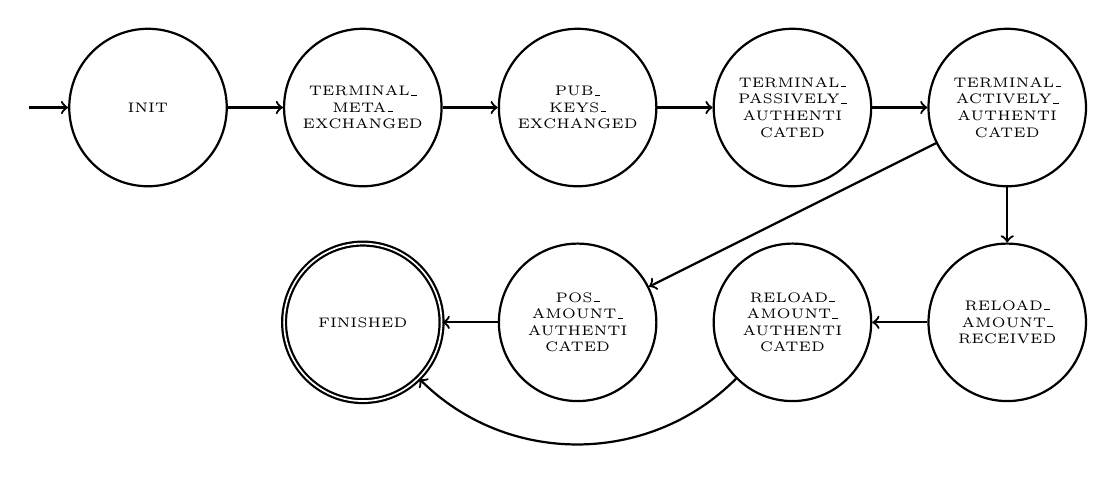
\begin{tikzpicture}[node distance=7mm and 7mm, thick, font=\tiny, end/.style = {main, double}, main/.style = {draw, circle, align=center, minimum size=2cm}]
\coordinate (start);

\node[main] (init) [right=0.5cm of start]{INIT};
\node[main] (metaExchanged) [right=of init] {TERMINAL\_\\META\_\\EXCHANGED};
\node[main] (keysExchanged) [right=of metaExchanged] {PUB\_\\KEYS\_\\EXCHANGED};
\node[main] (passivAuth) [right=of keysExchanged] {TERMINAL\_\\PASSIVELY\_\\AUTHENTI\\CATED};
\node[main] (activeAuth) [right=of passivAuth] {TERMINAL\_\\ACTIVELY\_\\AUTHENTI\\CATED};
\node[main] (reloadAmount) [below=of activeAuth] {RELOAD\_\\AMOUNT\_\\RECEIVED};
\node[main] (reloadAmountAuth) [left=of reloadAmount] {RELOAD\_\\AMOUNT\_\\AUTHENTI\\CATED};
\node[main] (PosAmountAuth) [left=of reloadAmountAuth] {POS\_\\AMOUNT\_\\AUTHENTI\\CATED};
\node[end] (finish) [left=of PosAmountAuth] {FINISHED};

\draw[->] (start) -- (init);
\draw[->] (init) -- (metaExchanged);
\draw[->] (metaExchanged) -- (keysExchanged);
\draw[->] (keysExchanged) -- (passivAuth);
\draw[->] (passivAuth) -- (activeAuth);
\draw[->] (activeAuth) -- (reloadAmount);
\draw[->] (reloadAmount) -- (reloadAmountAuth);
\draw[->] (activeAuth) -- (PosAmountAuth);
\draw[->] (PosAmountAuth) -- (finish);
\draw[->] (reloadAmountAuth) to [bend left=45] (finish);
\end{tikzpicture}
    \caption{State machine of the card, ensuring that no messages can be played out of sequence}
    \label{fig:stateMachine}
\end{figure}

\subsection{Blocking} \label{sec:blocking}
The following describes the blocking procedure of terminals and cards needed to comply with \ref{sr:block}.

\subsubsection{Terminals} \label{sec:blockTerminal}
The certificates for terminals are only issued for a rather short period of time, for example, one week.
This enforces the terminal to connect to the back end periodically.
By not issuing a new certificate for a terminal, the terminal is blocked.
This assumes that the clock provided by the terminal is genuine.
If it is not, a terminal can use an old certificate and just provide some clock signal that is within the validity range of this old certificate.

Another case the terminal is blocked temporarily occurs if the terminal counter used in the reload and payment protocols in figures~\ref{fig:POSProtocol} and \ref{fig:ReloadProtocol} would overflow.
To ensure that signature $S_1$ is still unique, the terminal needs a new certificate with a new expiration date.
Therefore, the terminal blocks itself until it got a new certificate.
After each certificate refresh, the counter is reset to zero.

\subsubsection{Cards} \label{sec:blockCards}
The cards can reach their end-of-live by different means.
The normal case would be that the certificate on the card expired.
As we trust the clock signal of the terminals, the card can check if it is expired and put its state to blocked in that case.

Similarly, we can set the state of some card to End-of-Live in the backend as soon as the certificate expired, as we can be sure that the card will block itself as soon as it would be used again.

Another way the card can get blocked is by revoking the certificate through a certificate revocation list (CRL) which is containing the following:
\begin{itemize}
    \item The list of all card IDs that got revoked,
    \item an expiration date,
    \item and a signature of the above, signed by the back end.
\end{itemize}
This would be helpful if the card gets lost or stolen.
The card would get blocked in the backend, which periodically distributes the CRL.
The POS and reload terminals will receive an update of that CRL every time they connect to the back end.
As shown in Step~\ref{seq:RELVerifCardCert} in the payment and reload protocol, the terminals check if the certificate of the card is revoked by the most recent CRL\@.
Preferably, the CRLs are distributed as soon as possible. 
However, there is a trade-off between being able to operate offline and blocking cards as soon as possible.

If a card that is on the CRL connects to a terminal, the terminal will send a message signed by the itself to the card to block itself.
After that, the card blocks locally and sends back a signed confirmation.
This confirmation is stored in the log of the terminal and (later) synchronized to the back end.
As the back end now knows that the card is blocked and cannot be unblocked again, it can delete the card ID from upcoming CRLs in order to keep it short.
In case the card is never used again after it was marked lost or stolen, the CRL entry will be kept until the certificate of the card is expired.

The last way a card can enter the blocked state is by an exhaustion of the counter used.
As described in the payment and reload protocols in figures~\ref{fig:POSProtocol} and \ref{fig:ReloadProtocol} this counter is continuously increased to prevent replay attacks.
As soon as this counter reaches its maximum value, the card will block to prevent the reuse of the counter, functioning as a nonce.

\section{Changes Since Last Version}
    \subsection{Personalization Protocol}
    In the original proposal, we wanted to send the public key of the back end together with the expiration date and card ID in one APDU\@.
    As the used RSA key is already 256 bytes in size, it fills up the whole APDU and thus we needed to split up the messages into two (steps~\ref{seq:InitBackendKeyToCard} and~\ref{seq:InitIdAndDateToCard}).

    \subsection{Reload and Payment Protocol}
    As with the personalization protocol, we experienced the limitation of the APDU size with the reload and payment protocol.
    We therefore split up the sending of certificates into three messages each (metadata, public key, and signature).
    Additionally, when sending signed information such an amount of money, we first send the information and then the signature in a separate message.

\end{document}
